\documentclass{standalone}
\usepackage{tikz}
\usetikzlibrary{shapes.geometric, positioning}

\begin{document}

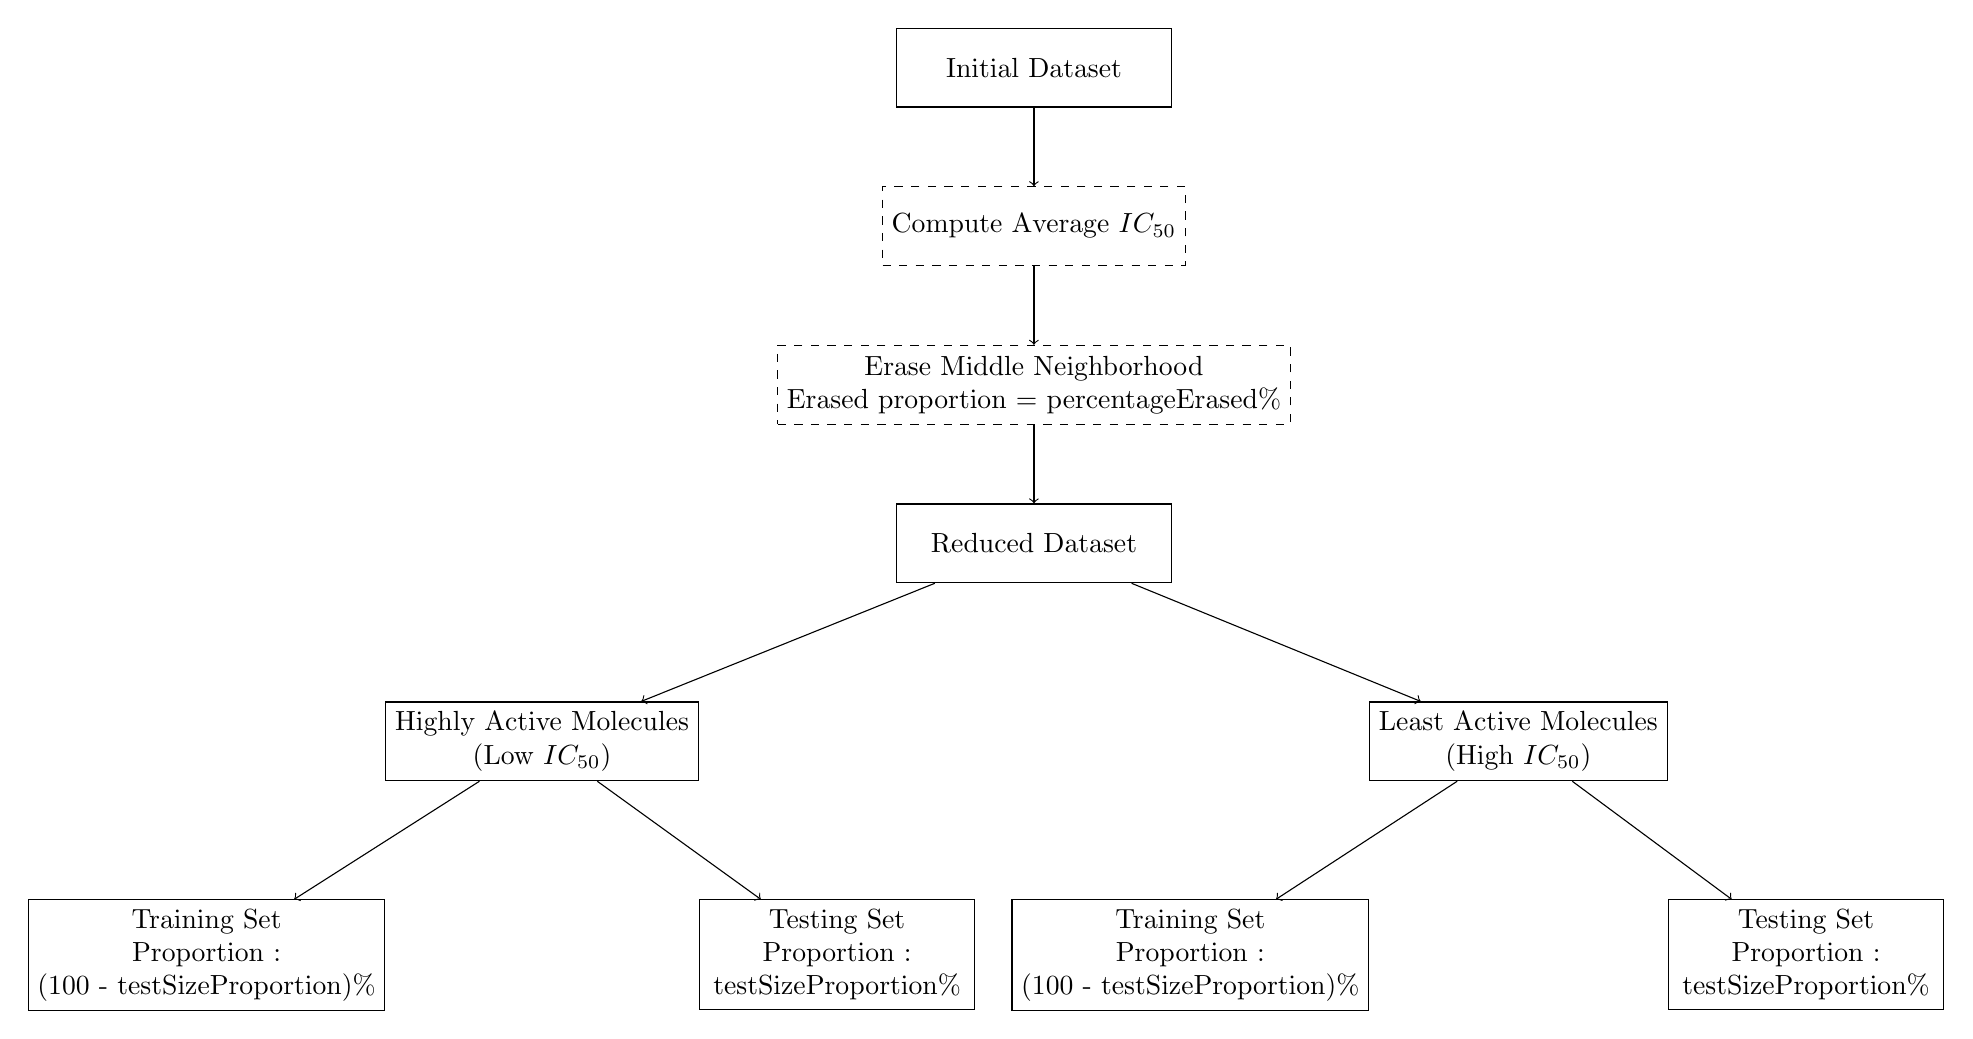
\begin{tikzpicture}[
    node distance=1.0cm and 0.5cm,
    every node/.style={draw, align=center, minimum width=3.5cm, minimum height=1.0cm},
    initialdataset/.style={rectangle},
    process/.style={rectangle, dashed},
    dataset/.style={rectangle},
    split/.style={rectangle},
    erased/.style={rectangle, dashed}
]

    % Initial dataset
    \node[initialdataset] (data) {Initial Dataset};

    % Compute Average IC50
    \node[process, below=of data] (average) {Compute Average $IC_{50}$};
    % Erased Neighborhood
    \node[erased, below=of average] (preerased) {Erase Middle Neighborhood \\ Erased proportion = percentageErased\%};
    
    \node[rectangle, below=of preerased] (erased) {Reduced Dataset};
    
    % Split into highly active and least active
    \node[split, below left=1.5cm and 2.5cm of erased] (highly) {Highly Active Molecules \\ (Low $IC_{50}$)};
    \node[split, below right=1.5cm and 2.5cm of erased] (least) {Least Active Molecules \\ (High $IC_{50}$)};

    % Training and Testing Splits
    \node[dataset, below left=1.5cm and 0cm of  highly] (high_train) {Training Set \\ Proportion :\\ (100 - testSizeProportion)\%};
    \node[dataset, below right=1.5cm and 0cm of  highly] (high_test) {Testing Set \\ Proportion :\\ testSizeProportion\%};

    \node[dataset, below left=1.5cm and 0cm of least] (low_train) {Training Set \\ Proportion :\\ (100 - testSizeProportion)\%};
    \node[dataset, below right=1.5cm and 0cm of least] (low_test) {Testing Set \\  Proportion :\\ testSizeProportion\%};

    % Arrows
    \draw[->] (data) -- (average);
    \draw[->] (average) -- (preerased);
    \draw[->] (preerased) -- (erased);
    \draw[->] (erased) -- (highly);
    \draw[->] (erased) -- (least);
    \draw[->] (highly) -- (high_train);
    \draw[->] (highly) -- (high_test);
    \draw[->] (least) -- (low_train);
    \draw[->] (least) -- (low_test);

\end{tikzpicture}

\end{document}